\begin{table}[t]
\centering
\label{tab:rmse_selected_leads}
\setlength{\tabcolsep}{3.5pt} % tighten column spacing
\renewcommand{\arraystretch}{1.15}
\begin{tabular}{rcccccc}
\toprule
Lead & XRO & \shortstack{NXRO\\Attn} & \shortstack{NXRO\\GNN} & \shortstack{NXRO\\MLP} & \shortstack{Neural\\ODE} & \shortstack{Trans\\former} \\
\midrule
3  & 0.350 & 0.289 & 0.298 & \textbf{0.275} & 0.401 & 0.406 \\
6  & 0.558 & 0.456 & 0.479 & \textbf{0.440} & 0.628 & 0.622 \\
9  & 0.659 & 0.571 & 0.598 & \textbf{0.571} & 0.718 & 0.749 \\
12 & 0.704 & \textbf{0.659} & 0.682 & 0.672 & 0.786 & 0.858 \\
15 & 0.763 & \textbf{0.740} & 0.750 & 0.778 & 0.859 & 0.948 \\
18 & 0.809 & 0.787 & \textbf{0.785} & 0.851 & 0.872 & 0.987 \\
21 & 0.833 & 0.807 & \textbf{0.801} & 0.883 & 0.856 & 0.968 \\
\midrule
Parameters & 650 & 633 & 537 & 6334 & 5514 & $\sim$ 170K \\ 
\bottomrule
\end{tabular}
\caption{RMSE at selected lead times  for the models explored in Figure \ref{fig:1c_core_models_ranking}. Best (lowest) RMSE per row is in bold. We see a clear pattern that MLP based nonlinear component performs the best at short-term, while attention starts to pick up at medium-term, and GNN at long-term. Overall all the NXRO variants consistently outperform the XRO baseline and the purely non-physical models.}
\end{table}

\begin{figure}
    \centering
    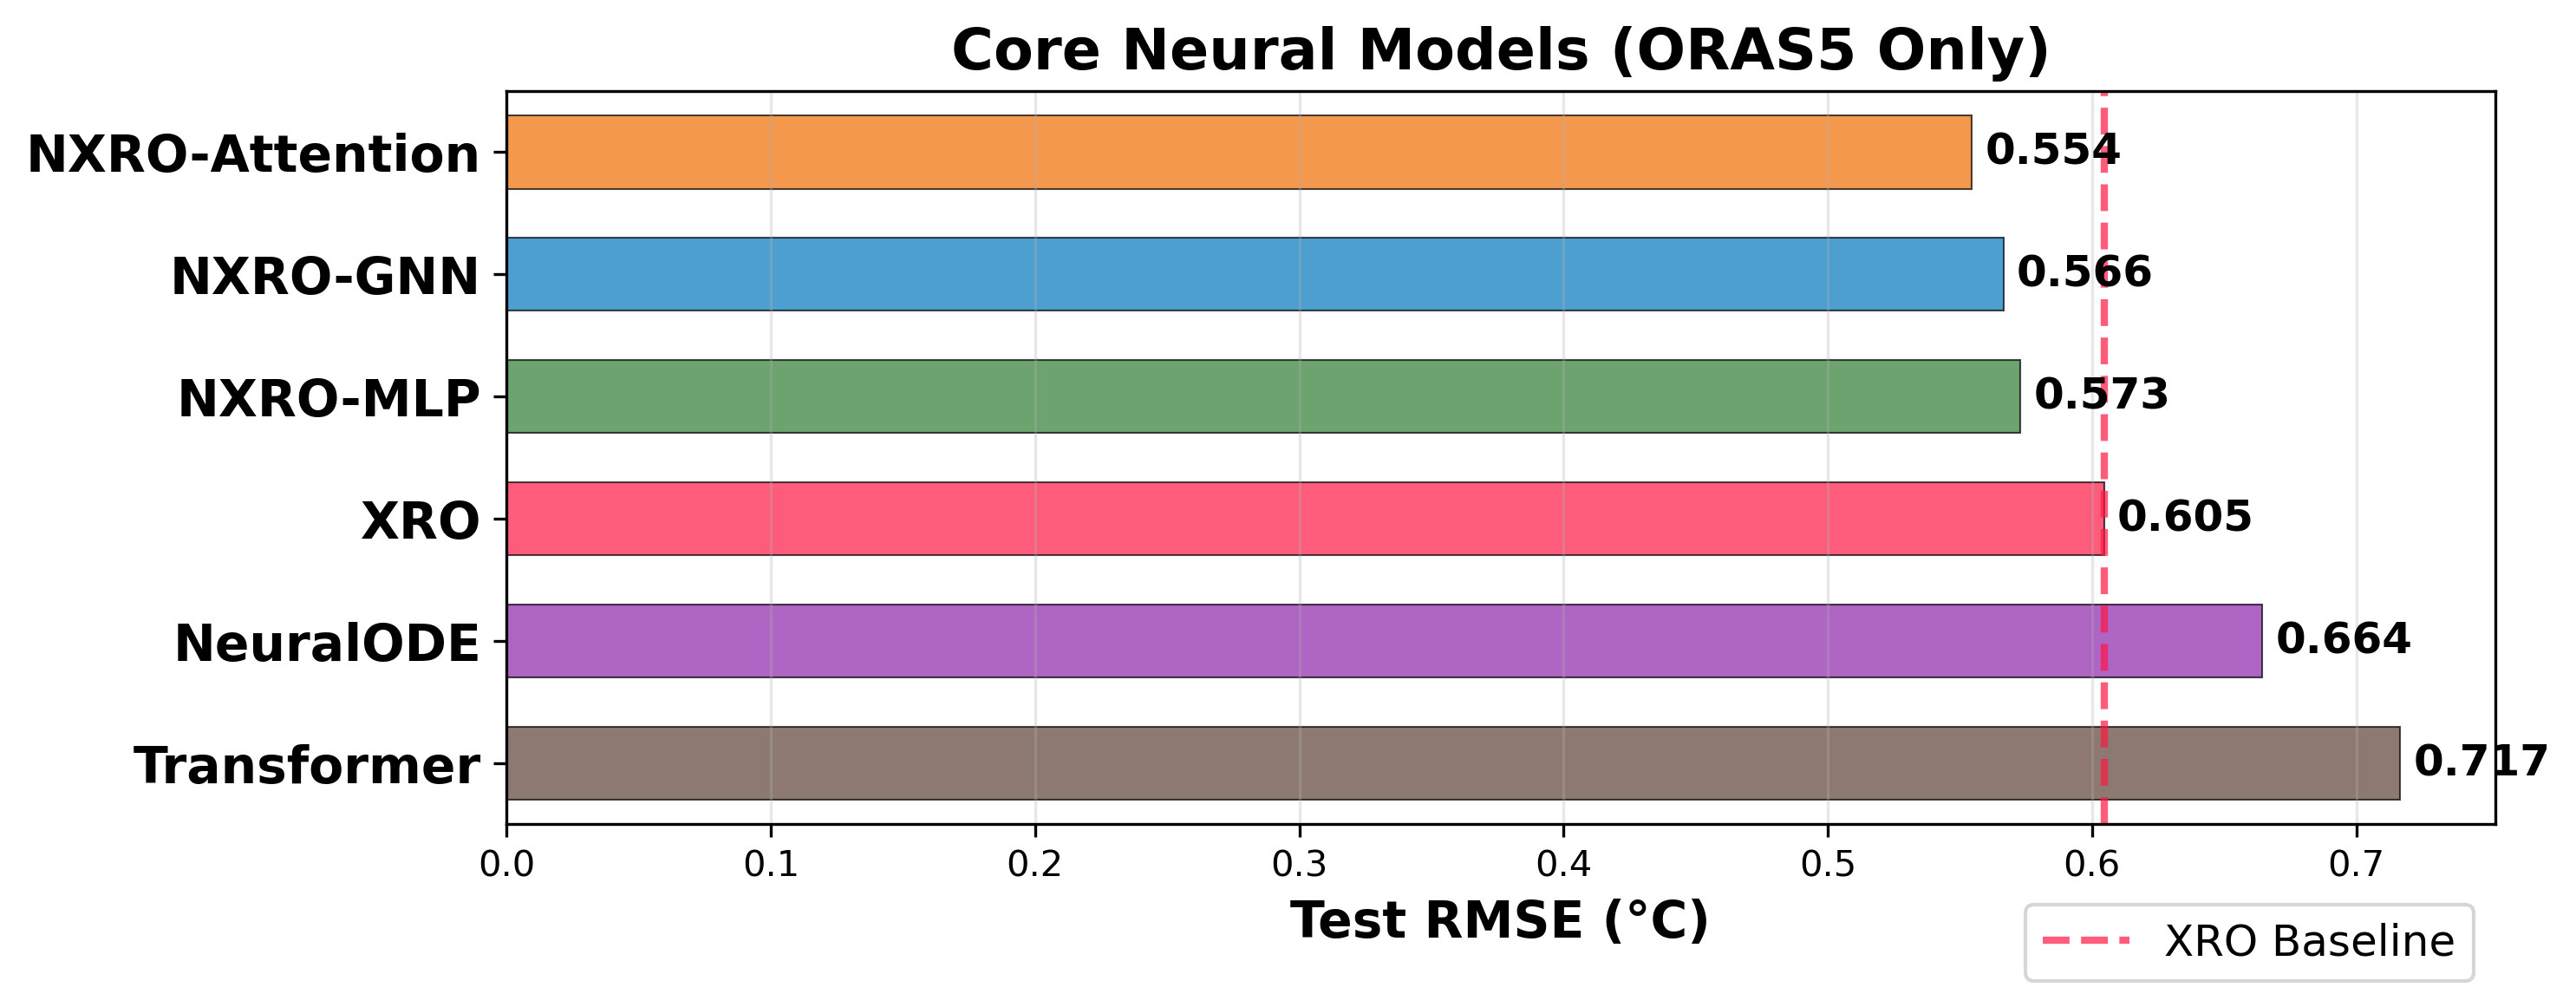
\includegraphics[width=\columnwidth]{figures/1c_core_models_ranking.png}
    \caption{Average RMSE across 21 lead times on the out-of-distribution ENSO forecast. NXRO variants outperform baselines by a significant margin.}
    \label{fig:1c_core_models_ranking}
\end{figure}